\documentclass[preprint,12pt,authoryear]{elsarticle}
\usepackage[a4paper,margin=25mm]{geometry}
\usepackage[T1]{fontenc}
\usepackage[utf8]{inputenc}
\usepackage{lmodern,microtype,amsmath,amssymb,graphicx,booktabs,tabularx}
\usepackage{url,xurl}
\usepackage[hidelinks]{hyperref}
\emergencystretch=2em
\hypersetup{pdftitle={Scenario-wise assessment of sparse virtual sensing and interpretable severity screening in simulated tunnel fires},pdfauthor={Heloi Moacyr Tanoue and Saulo Jose de Castro Almeida}}
\journal{Engineering Applications of Artificial Intelligence}
\begin{document}
\begin{frontmatter}
\title{Scenario-wise assessment of sparse virtual sensing and interpretable severity screening in simulated tunnel fires}
\author[unicamp]{Heloi Moacyr Tanoue\corref{cor}}
\ead{h231761@dac.unicamp.br}
\author[unicamp]{Saulo Jos\'e de Castro Almeida}
\ead{saulojca@unicamp.br}
\cortext[cor]{Corresponding author.}
\address[unicamp]{Faculty of Civil Engineering, Architecture and Urbanism, University of Campinas, Campinas, Brazil}
\begin{abstract}
Sparse monitoring requires an assessment of what can be inferred at locations
without measurements. This computational study evaluates contemporaneous
reconstruction of temperature, visibility and carbon monoxide at six omitted
virtual measurement sites using four observed sites. Nine corrected
computational fluid dynamics (CFD) cases span all combinations of three fire
powers (5, 10 and 20 MW) and three inlet-speed magnitudes (1, 2 and 3 m/s).
Six cases form a development set for leave-one-scenario-out comparison; three
other cases were reserved and evaluated once after the protocol was frozen.
Nearest-site and spatial-linear estimates are compared with Ridge and
random-forest regression. On the reserved cases, equal-scenario mean absolute
error (MAE) after output projection was lowest for spatial interpolation in
temperature (5.49 $^{\circ}$C), random forest in visibility (0.369 m), and
Ridge in carbon monoxide (2.05 ppm). However, Ridge's raw mean CO MAE was
2.80 ppm, and output projection changed 24.98\% of its CO estimates on
average. No method was consistently best across quantities. A separate
four-band local research rule showed high random-forest agreement in two
class-imbalanced cases, but it is not validated as a human-safety or alarm
criterion. The study supports a reproducible scenario-wise comparison, not
general ML superiority, physical validation or operational risk prediction.
\end{abstract}
\begin{keyword}
Tunnel fires \sep Virtual sensing \sep Sparse reconstruction
\sep Scenario-wise evaluation \sep Interpretable severity \sep Reproducibility
\end{keyword}
\end{frontmatter}

\section{Introduction}
Tunnel-fire monitoring must distinguish available observations from inferred
conditions at unobserved locations. In a numerical investigation, a virtual
sensor is a sampling location in a computed field. Removing some of those
locations from a model's inputs creates a testable reconstruction problem:
the omitted numerical measurements can be retained as evaluation targets.
This is more informative about reconstruction than asking a classifier to
recover labels calculated deterministically from its own input variables.
Neither task, by itself, validates fire consequences for occupants.

Simulation-derived fire databases and intelligent monitoring systems are
established research directions \citep{Zhang2021TunnelDatabase,Wu2022TunnelFirefighting}.
Limited ceiling-temperature data have been used for full-field reconstruction
\citep{Guo2024LimitedTemperature}, while transfer learning has been evaluated
for fire-source inversion using numerical and physical observations
\citep{Jiang2025TransferTunnel}. Online sparse measurements also support
physics-informed temperature reconstruction and prediction
\citep{Jiang2026PhysicsInformed}. Thus, combining simulation, virtual sensors
and a learning model is not itself a research gap.

The specific question addressed here is whether conventional regressors
improve contemporaneous reconstruction over transparent spatial estimates
when entire CFD scenarios, rather than randomly selected time rows, are
withheld. The study uses a fixed four-observed/six-omitted site layout and a
crossed 3-by-3 set of fire-power and inlet-speed conditions. Six scenarios
support development comparisons; three are kept as a final reserved set.
Reconstruction errors are also examined through a separate local research
severity rule. The scope is a CFD-based feasibility assessment, not a claim
to have solved sparse tunnel-fire monitoring.

The contributions are (i) a traceable, crossed set of corrected CFD cases
with an explicit development/reserved partition, (ii) a scenario-wise
comparison of two learned regressors with nearest-site and spatial-linear
baselines under a fixed sensor layout, and (iii) a transparent assessment of
how reconstruction and unsupported inputs affect a separately defined local
severity interpretation. The study retains unfavorable results and reports
raw as well as bounded predictions where output projection changes them.
It does not introduce a new learning algorithm, demonstrate general ML
superiority, validate full-field reconstruction, or evaluate forecasting,
multi-agent coordination or closed-loop ventilation control.

\section{Related work and scope}
\citet{Guo2024LimitedTemperature} investigate reconstruction of tunnel
temperature distributions from limited monitored ceiling-flow information.
\citet{Jiang2025TransferTunnel} address inversion of source location and
heat release using transfer learning and reduced- and full-scale fire
observations. \citet{Jiang2026PhysicsInformed} investigate a physics-informed
neural network with online sparse monitoring. These studies establish
precedents for sparse sensing and for substantially broader validation
than is available here. Their prediction targets, data and experimental
designs differ; their reported scores are not direct benchmarks for the
present task. Here, the narrower methodological question is multi-quantity,
contemporaneous reconstruction at fixed unobserved sites, with fitted
regressors evaluated against spatial baselines under complete-scenario
holdout and a separate local-rule analysis. This defines the scope of the
comparison rather than asserting that sparse tunnel-fire sensing is an
unexplored topic. The literature positioning relies on the accessible
publisher abstracts and article metadata; it does not claim a
reimplementation of those methods.

An intelligent tunnel-fire system with a small-scale demonstration is
reported by \citet{Wu2022TunnelFirefighting}; broader database and artificial
intelligence opportunities are discussed by \citet{Zhang2021TunnelDatabase}.
The present contribution is limited to a reproducible benchmark and its
failure diagnosis. Standard Ridge and random-forest models are used as
comparators, not presented as newly developed methods.

Risk assessment also requires a different evidential basis from a local
condition score. The PIARC Road Tunnels Manual treats risk assessment as
a structured analysis of scenarios and consequences
\citep{PIARCRiskAssessment}. The official scope of ISO 13571 concerns time
to compromised tenability from fire components \citep{ISO13571Scope}.
Here, no occupant trajectory, exposure integration or event probability
is modeled. The term \emph{severity screening} therefore denotes a
research interpretation of local simulated quantities, not a validated
probability of harm or an evacuation criterion.

\section{Corrected simulation data}
\subsection{Configuration and provenance}
Nine production runs use Fire Dynamics Simulator version 6.8.0,
revision \texttt{886e009}. The computational extent is 50~m longitudinally,
7.25~m vertically and 13.25~m transversely, with four meshes and uniform
0.25~m cells (307,400 cells in total). Coordinates are explicitly defined
as longitudinal $x$, upward $y$ and transverse $z$; the configured gravity
is $(0,-9.81,0)$~m/s$^2$ and ambient temperature is $20\,^{\circ}$C.
These are an idealized tunnel-section model, not measurements of an
operating immersed tunnel.

The 10~m$^2$ floor burner occupies $24\leq x\leq26$~m and
$-2.5\leq z\leq2.5$~m. Prescribed heat release per unit area is
500, 1000 or 2000~kW/m$^2$, respectively. The ramp factors are 0 at
0~s, 0.25 at 30~s and 1 at 60~s, with the final value maintained to
600~s. An upstream supply and downstream open boundary prescribe
inlet-speed magnitudes of 1, 2 and 3~m/s. The supply-normal velocities
in the decks are negative, as required for these inlet faces.

The reaction specifies n-heptane, soot yield 0.05, carbon monoxide yield
0.01 and radiative fraction 0.35. Concrete surfaces use density
2200~kg/m$^3$, conductivity 1.7~W/(m K), specific heat
0.88~kJ/(kg K), thickness 0.20~m and insulated backing. These are
prescribed modeling assumptions, not calibrated material or combustion
measurements. Visibility is a simulator-derived quantity with a 30~m
output cap \citep{FDS680Criteria}. Carbon monoxide volume fraction is
converted to parts per million by multiplication by $10^6$.

\begin{table}[htbp]\centering\small
\caption{Corrected CFD cases in the crossed 3-by-3 design. Mean achieved
heat release is computed over 300--600~s. The reserved cases were evaluated
only after the analysis protocol was frozen.}
\label{tab:cases}
\begin{tabular}{@{}lrrrl@{}}\toprule
Case & Power (MW) & Inlet (m/s) & Mean HRR (MW) & Partition\\
\midrule
S1      & 5  & 1 & 5.00022  & Development\\
P05V02  & 5  & 2 & 5.00017  & Development\\
P05V03  & 5  & 3 & 5.00039  & Reserved\\
P10V01  & 10 & 1 & 10.00083 & Reserved\\
S2      & 10 & 2 & 10.00016 & Development\\
P10V03  & 10 & 3 & 10.00082 & Development\\
P20V01  & 20 & 1 & 20.00131 & Development\\
P20V02  & 20 & 2 & 20.00321 & Reserved\\
S3      & 20 & 3 & 20.00195 & Development\\\bottomrule
\end{tabular}
\end{table}

The cases form all nine combinations of the three prescribed fire powers
and three inlet-speed magnitudes. This crossed design prevents the original
one-to-one pairing of power and ventilation from defining the expanded
dataset; it does not constitute a broad uncertainty study or validation
outside the modeled geometry and source configuration.

The selected inputs correct the earlier ambient-temperature and gravity-axis
inconsistencies. A separate rerun also corrects an earlier nominal-20-MW
S3 deck whose burner actually prescribed 30~MW. That 30~MW run is preserved
as an excluded archive, not included in Table~\ref{tab:cases}. Input
hashes, solver logs, achieved heat release, channel units, finite-value
checks and time coverage link the chosen files to the analysis. Solver
completion and these consistency checks do not constitute independent
physical validation. No mesh-convergence or physical fire test is reported.

\subsection{Sites, channels and sampling}
Ten sites form pairs at $x=15,20,25,30,35$~m with
$y=6.8$~m and $z=\pm3$~m. Each site supplies temperature $T$,
visibility $V$, carbon monoxide concentration $C$ and longitudinal
velocity $U$. Thus, ten \emph{sites} correspond to forty article
measurement channels; six additional passive diagnostic devices are
excluded from the regression inputs and targets. Devices sample
computed local fields, without a physical sensor-response model.

The four observed sites are S01, S02, S09 and S10, at $x=15$ and 35~m.
The six internal sites S03--S08, at $x=20,25,30$~m, are omitted from
the predictors and retained as numerical targets
(Fig.~\ref{fig:layout}). Each case contains 601 timestamps from
0 to 600~s; nominal one-second device output is slightly irregular.
The analysis uses the recorded timestamps and contemporaneous channels
without temporal interpolation, derivatives or future values.

\begin{figure}[htbp]\centering
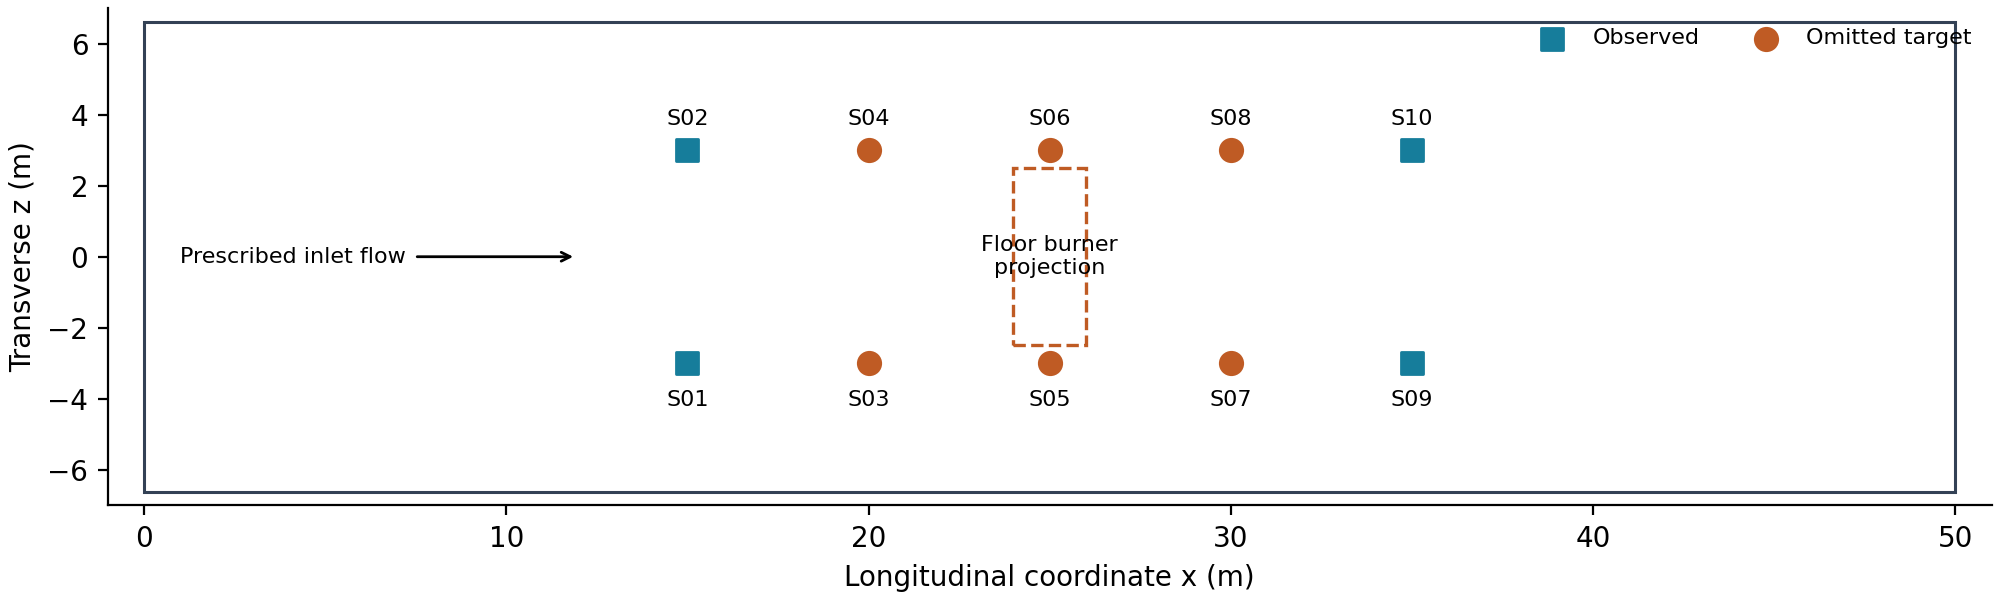
\includegraphics[width=\linewidth]{figures/site-layout.png}
\caption{Observed and omitted sites at $y=6.8$~m in longitudinal--transverse
view. The floor burner is shown as a projected footprint. This is a
numerical layout, not an as-built instrumentation drawing.}
\label{fig:layout}
\end{figure}

\section{Fixed reconstruction benchmark}
\subsection{Inputs and separation}
For target site $j$ and timestamp $t$, the input is
\begin{equation}
\mathbf{x}_{jt}=\big[(T,V,C,U)_{a,t}:a\in\mathcal{O};\;x_j,z_j\big],
\qquad \widehat{\mathbf{q}}_{jt}=f(\mathbf{x}_{jt}),
\end{equation}
where $\mathcal{O}$ contains the four observed sites and
$\mathbf{q}_{jt}=(T,V,C)_{jt}$. There are 18 features: 16 observed channel
values and two target coordinates. Scenario identity, nominal heat release,
prescribed inlet speed, elapsed time and all omitted-site measurements are
excluded as predictors. Measured $U$ remains available as flow context.

Evaluation has two scenario-wise stages. During development, each of the
six development cases is withheld in turn; five cases provide 18,030
training target--time rows and the withheld case provides 3,606 test rows.
No random row split is used. After these comparisons, the final protocol
was frozen and the three reserved cases in Table~\ref{tab:cases} were
evaluated once, each using all six development cases for training
(21,636 target--time rows) and 3,606 test rows. Training-only transformations
precede test prediction. All six target coordinates occur in the training
cases, so this protocol does not test new target positions or a new geometry.
There are nine numerical fire runs, not 32,454 independent experiments;
repeated times and sites are correlated observations within each run.

The development and reserved protocols, input hashes and case assignments
are archived. The final evaluation specification was frozen before the
reserved histories were opened. This is an internal design record, not an
external preregistration. No hyperparameter search or post-holdout model
selection was performed.

\subsection{Comparators}
The nearest-site estimate uses the closest observed longitudinal endpoint
on the same transverse side, taking the upstream point on a tie. Linear
interpolation uses the two same-side observed endpoints:
\begin{equation}
\widehat q_j=(1-\lambda_j)q_{15}+\lambda_j q_{35},
\qquad \lambda_j=(x_j-15)/20.
\end{equation}
These comparators require no fitting and use the same available observation
layout, although only the corresponding channel is needed.

Ridge uses training-only standardization and regularization parameter
$\alpha=1$. The random forest uses 100 trees, maximum depth 10, minimum
leaf size 5, seed 42 and one worker. Each learned method fits one regressor
per output quantity. These fixed settings were used in both the six-fold
development comparison and the final fits; implementations use
scikit-learn 1.7.2.

All methods receive identical output projection: $T\geq-273.15\,^{\circ}$C,
$0\leq V\leq30$~m and $0\leq C\leq10^6$~ppm. Projection frequencies
are recorded. These representational bounds are not a physics-informed
loss, a calibrated physical constraint or a reliability mechanism.
They cannot make an unstable model acceptable.

For the final applicability screen, a target--time estimate is marked
available only when all 18 input features lie within their training-set
minima and maxima. The same rule is applied to all four methods. This
feature-wise screen does not establish joint-distribution support or
safety; estimates outside it are reported as unavailable for the screening
interpretation, not as Low. Regression errors are retained both across all
rows (as extrapolation diagnostics) and within the supported subset.

\subsection{Metrics}
For each test scenario, quantity and method, mean absolute error (MAE),
root mean squared error, maximum absolute error, bias and $R^2$ are
computed against omitted simulator outputs. The same errors are retained
by site. Development and reserved results are summarized separately; in
each stage, the principal summary gives equal weight to each scenario's
MAE for each quantity. Raw and projected model outputs are retained.
Incompatible physical units are not combined into a single error. No
row-based significance test or claim of thousands of independent examples
is made. Agreement with withheld simulator values evaluates reconstruction
of this CFD model, not accuracy against physical tunnel conditions.

\section{Separate interpretable severity definition}
\label{sec:severity}
The research definition \texttt{local-severity-research-2.0} revises the
former three-class article implementation. Temperature, visibility and
carbon monoxide band boundaries are listed in Table~\ref{tab:bands}.
They follow the four-class methodological criteria in the authors'
confirmed final dissertation. They are not asserted to be universal
tenability limits or requirements of a fire-safety standard. The maximum
aggregation specified here is an explicit new design choice because the
earlier descriptions did not uniquely determine mixed-indicator cases.

\begin{table}[htbp]\centering
\caption{Research band transitions (0=Low, 1=Medium, 2=High, 3=Critical).
Equality enters the higher band. The names denote this rule's outputs.}
\label{tab:bands}
\begin{tabular}{@{}lccc@{}}\toprule
Quantity & Enter band 1 & Enter band 2 & Enter band 3\\\midrule
$T$ ($^{\circ}$C) & $\geq40$ & $\geq80$ & $\geq150$\\
$V$ (m) & $\leq20$ & $\leq10$ & $\leq5$\\
$C$ (ppm) & $\geq50$ & $\geq200$ & $\geq800$\\\bottomrule
\end{tabular}
\end{table}

Define component bands as
\begin{align}
b_T&=\sum_{a\in\{40,80,150\}}\mathbf{1}(T\geq a), &
b_V&=\sum_{a\in\{20,10,5\}}\mathbf{1}(V\leq a),\\
b_C&=\sum_{a\in\{50,200,800\}}\mathbf{1}(C\geq a), &
b&=\max(b_T,b_V,b_C).
\end{align}
No benign channel can cancel a higher component band. Velocity is
context, rather than a universally monotonic hazard indicator.

A separate gradual index $g=\max(g_T,g_V,g_C)$ uses piecewise-linear,
saturated functions through the points
\begin{align}
g_T &: (20,0),(40,1/3),(80,2/3),(150,1),\\
g_V &: (5,1),(10,2/3),(20,1/3),(30,0),\\
g_C &: (0,0),(50,1/3),(200,2/3),(800,1).
\end{align}
This is fuzzy-inspired gradual normalization with a maximum operator;
it is not a Mamdani rule system or a new fuzzy-inference algorithm.
No new numerical weights are introduced. Missing or invalid measurements
are rejected instead of being mapped to the lowest band.

The same rule is applied to withheld and reconstructed quantities.
Band agreement, underestimation frequency, highest-band misses and
gradual-index MAE describe the effect of reconstruction on this research
rule. The rule is not the supervised regression target. Its labels remain
methodological references, not independently observed fire-risk ground truth.
Sampling at 6.8~m does not establish occupant breathing-zone conditions;
maximum CO is not an integrated toxic dose.

\section{Results}
\subsection{Development comparison across six scenarios}
Table~\ref{tab:development-mae} gives the equal-scenario mean of the six
leave-one-scenario-out MAEs after the shared output projection. The
nearest-site estimate has the lowest development MAE for visibility and
CO, while its temperature MAE is effectively tied with interpolation.
The random forest has lower MAE than spatial interpolation in only two
of six folds for each quantity. Its temperature MAE reaches 109.92~$^{\circ}$C
when P20V01 is withheld, compared with 14.82~$^{\circ}$C for interpolation.
This case also has substantial range extrapolation: 91.85\% of its
target--time rows have at least one input outside the training min--max
range. The screen's development coverage for P20V01 is 8.15\%; this
motivated retaining an explicit availability flag, but does not validate
the screen as a safety mechanism.

\begin{table}[htbp]\centering\small
\caption{Development-stage mean MAE across six leave-one-scenario-out
folds, giving equal weight to each complete scenario. Shared output
projection is applied; quantities retain separate units.}
\label{tab:development-mae}
\begin{tabular}{@{}lrrr@{}}\toprule
Method & $T$ ($^{\circ}$C) & $V$ (m) & $C$ (ppm)\\\midrule
Nearest site & 9.86 & 2.97 & 3.21\\
Spatial linear & 9.85 & 3.89 & 3.67\\
Ridge & 15.22 & 6.81 & 4.78\\
Random forest & 30.07 & 4.73 & 9.62\\
\bottomrule
\end{tabular}
\end{table}

\subsection{One-time evaluation on the reserved scenarios}
Table~\ref{tab:reserved-mae} reports the projected MAE for each reserved
case against its omitted CFD measurements. Each case contributes 3,606
target--time pairs. The support screen marked 3,600/3,606 pairs available
for P05V03 (99.83\%) and all pairs available for P10V01 and P20V02.
These near-complete coverage values do not show that the input combinations
are jointly supported by the training distribution.

\begin{table}[htbp]\centering\small
\caption{MAE after the shared output projection on the reserved cases.
The regression diagnostics include all rows, including rows outside the
feature-wise support screen. Ridge raw and projected summaries are
discussed in the text.}
\label{tab:reserved-mae}
\begin{tabular}{@{}llrrr@{}}\toprule
Case & Method & $T$ ($^{\circ}$C) & $V$ (m) & $C$ (ppm)\\\midrule
P05V03 & Nearest site & 0.265 & 0.000 & $9.13\times10^{-10}$\\
P05V03 & Spatial linear & 0.181 & 0.000 & $1.37\times10^{-9}$\\
P05V03 & Ridge & 6.754 & 0.019 & 0.048\\
P05V03 & Random forest & 0.085 & 0.0003 & 0.0005\\
P10V01 & Nearest site & 9.738 & 0.723 & 3.573\\
P10V01 & Spatial linear & 7.103 & 0.663 & 3.489\\
P10V01 & Ridge & 6.404 & 2.622 & 2.515\\
P10V01 & Random forest & 15.245 & 0.448 & 5.700\\
P20V02 & Nearest site & 12.755 & 1.213 & 4.488\\
P20V02 & Spatial linear & 9.181 & 1.288 & 3.553\\
P20V02 & Ridge & 10.242 & 3.252 & 3.585\\
P20V02 & Random forest & 12.707 & 0.659 & 4.934\\
\bottomrule
\end{tabular}
\end{table}

Giving equal weight to the three reserved scenarios, spatial interpolation
has the lowest projected temperature MAE (5.49~$^{\circ}$C), random forest
the lowest visibility MAE (0.369~m), and Ridge the lowest projected CO MAE
(2.05~ppm). The Ridge CO result depends on projection: its raw equal-case
mean CO MAE is 2.80~ppm, compared with 2.05~ppm after projection; the
corresponding visibility MAE changes from 3.03 to 1.96~m. On P05V03,
projection modifies 99.67\% of Ridge visibility outputs and 72.55\% of
its CO outputs, reducing their MAEs from 3.049 to 0.019~m and from 2.277
to 0.048~ppm, respectively. P05V03 is almost entirely at the lower bounds
of the research rule, so these projected errors must not be interpreted
as evidence of a learned reconstruction advantage. The random forest is
better than spatial interpolation in 1/3 reserved cases for temperature,
2/3 for visibility, and 0/3 for CO. No method dominates across quantities.

\subsection{Effect on the local research severity rule}
The CFD references for P05V03 are Low at all 3,606 target--time pairs.
P10V01 contains 222/43/52/3,289 Low/Medium/High/Critical pairs, and P20V02
contains 368/8/12/3,218. Thus, Critical represents 91.2\% and 89.2\% of
the latter two cases, respectively; the high overall agreement in these
cases is influenced by this class imbalance. These are correlated local
samples, not independent events.

\begin{table}[htbp]\centering\small
\caption{Agreement with the local research rule on supported pairs after
output projection. Agreement, underestimation and Critical misses are
percentages; Critical misses use only reference-Critical pairs and are
undefined for P05V03. Gradual-index MAE is on the 0--1 scale.}
\label{tab:severity}
\begin{tabular}{@{}llrrrr@{}}\toprule
Case & Method & Agreement & Underest. & Critical miss & Gradual MAE\\\midrule
P05V03 & Nearest site & 100.00 & 0.00 & -- & 0.0044\\
P05V03 & Spatial linear & 100.00 & 0.00 & -- & 0.0030\\
P05V03 & Ridge & 99.94 & 0.00 & -- & 0.0065\\
P05V03 & Random forest & 100.00 & 0.00 & -- & 0.0014\\
P10V01 & Nearest site & 96.31 & 2.38 & 1.03 & 0.0193\\
P10V01 & Spatial linear & 96.73 & 2.44 & 1.00 & 0.0176\\
P10V01 & Ridge & 68.16 & 31.72 & 32.08 & 0.0545\\
P10V01 & Random forest & 98.64 & 0.83 & 0.40 & 0.0049\\
P20V02 & Nearest site & 95.48 & 3.16 & 3.39 & 0.0384\\
P20V02 & Spatial linear & 91.15 & 5.41 & 5.87 & 0.0401\\
P20V02 & Ridge & 58.18 & 39.10 & 43.51 & 0.0646\\
P20V02 & Random forest & 95.59 & 2.80 & 3.05 & 0.0167\\
\bottomrule
\end{tabular}
\end{table}

The random forest has the highest band agreement on the two cases with
multiple reference bands, with underestimation of 0.83\% and 2.80\% and
Critical misses of 0.40\% and 3.05\%, respectively. Ridge underestimates
the local band in 31.72\% and 39.10\% of supported pairs in those cases.
The random forest also has the lowest gradual-index MAE in each reserved
case, but this index is derived from the same local variables and rule;
it is not an independent fire-risk reference.
These results compare model outputs with the stated research rule; they
are not physical false-negative alarm rates. P05V03's 100\% agreement is
uninformative about discrimination because its reference contains only
the Low band. Neither agreement nor continuous MAE establishes decision
reliability.

\section{Discussion}
The six-case development comparison and one-time evaluation on three
reserved power--ventilation combinations provide a more informative test
than a random split of correlated time rows. Even so, the results do not
support general superiority of learned regression. Spatial interpolation
has the lowest reserved mean temperature MAE, the random forest the lowest
visibility MAE, and Ridge has the lowest CO MAE only after output
projection. The raw Ridge CO error is higher than the interpolation error,
and its visibility and CO estimates are materially changed by projection.
The relative ranking therefore depends on quantity, scenario and output
representation. Simple spatial baselines remain essential comparators and
are not validated substitutes for missing measurements.

The feature-wise min--max rule identified six unsupported pairs in P05V03
and none in the other reserved cases. This high coverage is not evidence
that all multivariate input combinations are familiar: separate feature
ranges cannot certify joint support, and the screen was not calibrated
against physical failure. A deployment would need an independently
validated applicability method and explicit handling of untrusted
estimates. In this study, ``unavailable'' is a reporting state, not an
implemented operational safeguard.

The severity analysis adds a separate decision-oriented view, but its
interpretation is limited. Critical references account for about 89--91\%
of the two reserved cases containing multiple bands, so overall agreement
is sensitive to class prevalence. Reporting underestimation and Critical
miss rates alongside agreement makes this limitation visible. The four
thresholds follow the authors' confirmed final dissertation, while the
maximum aggregation is an explicit methodological choice in this study.
Neither has been calibrated against occupant harm, exposure duration,
alarm performance or operational decisions. These are local research
bands, not validated risk, tenability or safety criteria.

The crossed grid separates the prescribed fire-power and inlet-speed
combinations more effectively than the earlier diagonal cases, but all
nine runs still share one idealized geometry, burner position, mesh
resolution, solver, reaction and boundary configuration. There is no
physical fire-test validation, mesh-convergence analysis, alternate
geometry, sensor-response model or assessment of noise, drift, missing
channels, alarm delay or false alarms. Omitting virtual inputs in
post-processing does not demonstrate a reduction in installed sensors.

The defensible contribution is a reproducible, scenario-wise comparison
and failure analysis for CFD-derived virtual sensing, with a transparent
local severity interpretation. The study does not establish algorithmic
novelty or a general AI benefit. Stronger engineering-AI claims would
require a justified inference advance and independent evidence that it
adds value over spatial baselines; adding untested agents or ventilation
control would not follow from the present results.

\section{Conclusion}
This study evaluated contemporaneous reconstruction of three CFD
quantities at six omitted virtual sites, using four observed sites and
nine crossed fire-power/inlet-speed cases. Six cases supported
leave-one-scenario-out development and three were evaluated once under a
frozen protocol. On the reserved cases, the best average method differed
by quantity, and Ridge's apparent CO advantage depended on output
projection. The random forest showed high agreement with the local
research severity rule in two class-imbalanced cases, but this rule is
not validated for human safety or operations. The results support a
reproducible comparative feasibility study; they do not establish general
ML superiority, physical validity or a novel inference algorithm.

Further work should evaluate applicability and failure handling on
independent CFD configurations and physical data, and test whether a
well-justified inference method provides measurable value beyond spatial
baselines before making operational or safety claims.

\section*{Data and code availability}
The accompanying reproducibility archive contains the nine selected input
decks, numerical device and heat-release outputs, execution logs, curated
data tables, frozen development and reserved protocols, analysis scripts,
result tables and software-version records. It excludes field-slice
binaries and the earlier invalid 30-MW S3 run, which remains separately
archived. No public repository DOI has yet been assigned to this revised
package. The supplied scripts use a portable package layout; no container
build or independent external replication is claimed.

\section*{Author contributions and disclosures}
Heloi Moacyr Tanoue: Methodology, Investigation, Software, Formal analysis,
Writing -- original draft. Saulo Jos\'e de Castro Almeida: Supervision,
Writing -- review and editing. The authors declare no competing interests.
Both authors reviewed and approved this substantially revised version. This
work was carried out with support from the National Council for Scientific
and Technological Development (CNPq), Brazil, under Funding Code
131754/2025-4. UNICAMP and CENAPAD-SP provided institutional and
computational support.

\section*{Declaration of generative artificial intelligence assistance}
OpenAI ChatGPT/Codex assisted with drafting, source inspection and writing
analysis code for this revision. The reconstruction quantities come from
the identified simulation files, and benchmark metrics were computed by
the supplied scripts. The retained site-layout figure is programmatically
drawn from the recorded coordinates; no generative image is used in this
version. Earlier GPT-5.0-assisted schematic figures are not reused. The
authors retain responsibility for verifying the code, results, references
and manuscript before submission.

\bibliographystyle{elsarticle-harv}
\bibliography{references}
\end{document}

